\Class{Rogue}
{Marek, always helpful, said that the UnderTyr catacombs are supposed to be haunted. Think I'll go make some inquiries about where a 'heretic' like me can get some holy earth. Always go prepared...}{Janos, human rogue}

{\tableheader Dark Sun} offers a world of intrigue, manipulation, secret deals, and subtle treachery---in short, a rogue's playground. Rather than eking out their living at the
borders of society, many Athasian rogues dominate the action in many of the most powerful political factions in the Seven Cities: the Noble Houses, the templars, and the Merchant Houses. Often rogues themselves, the wealthy and powerful deploy lesser rogues as pawns in their endless games of acquisition, espionage, and deceit.

Individual rogues run the gamut of Athasian society, from the street rats of the cities to the vagabonds of the outlands, to the prosperous and respectable dune traders, to the low-ranking templars that search their caravans at the gates. Accomplished rogues are often sought by the nobility as agents, and can earn both wealth and honor in such positions---or earn a quick death should they be caught contemplating treachery against their masters.

\WarriorTable{The Rogue}{
1 & +0 & +0 & +2 & +0 & Sneak attack +1d6, trapfinding\\
2 & +1 & +0 & +3 & +0 & Evasion\\
3 & +2 & +1 & +3 & +1 & Sneak attack +2d6, trap sense +1\\
4 & +3 & +1 & +4 & +1 & Uncanny dodge\\
5 & +3 & +1 & +4 & +1 & Sneak attack +3d6\\
6 & +4 & +2 & +5 & +2 & Trap sense +2\\
7 & +5 & +2 & +5 & +2 & Sneak attack +4d6\\
8 & +6/+1 & +2 & +6 & +2 & Improved uncanny dodge\\
9 & +6/+1 & +3 & +6 & +3 & Sneak attack +5d6, trap sense +3\\
10 & +7/+2 & +3 & +7 & +3 & Special ability\\
11 & +8/+3 & +3 & +7 & +3 & Sneak attack +6d6\\
12 & +9/+4 & +4 & +8 & +4 & Trap sense +4\\
13 & +9/+4 & +4 & +8 & +4 & Sneak attack +7d6, special ability\\
14 & +10/+5 & +4 & +9 & +4 & \\
15 & +11/+6/+1 & +5 & +9 & +5 & Sneak attack +8d6, trap sense +5\\
16 & +12/+7/+2 & +5 & +10 & +5 & Special ability\\
17 & +12/+7/+2 & +5 & +10 & +5 & Sneak attack +9d6\\
18 & +13/+8/+3 & +6 & +11 & +6 & Trap sense +6\\
19 & +14/+9/+4 & +6 & +11 & +6 & Sneak attack +10d6, special ability\\
20 & +15/+10/+5 & +6 & +12 & +6 & }

\begin{figure}[t!]
\centering
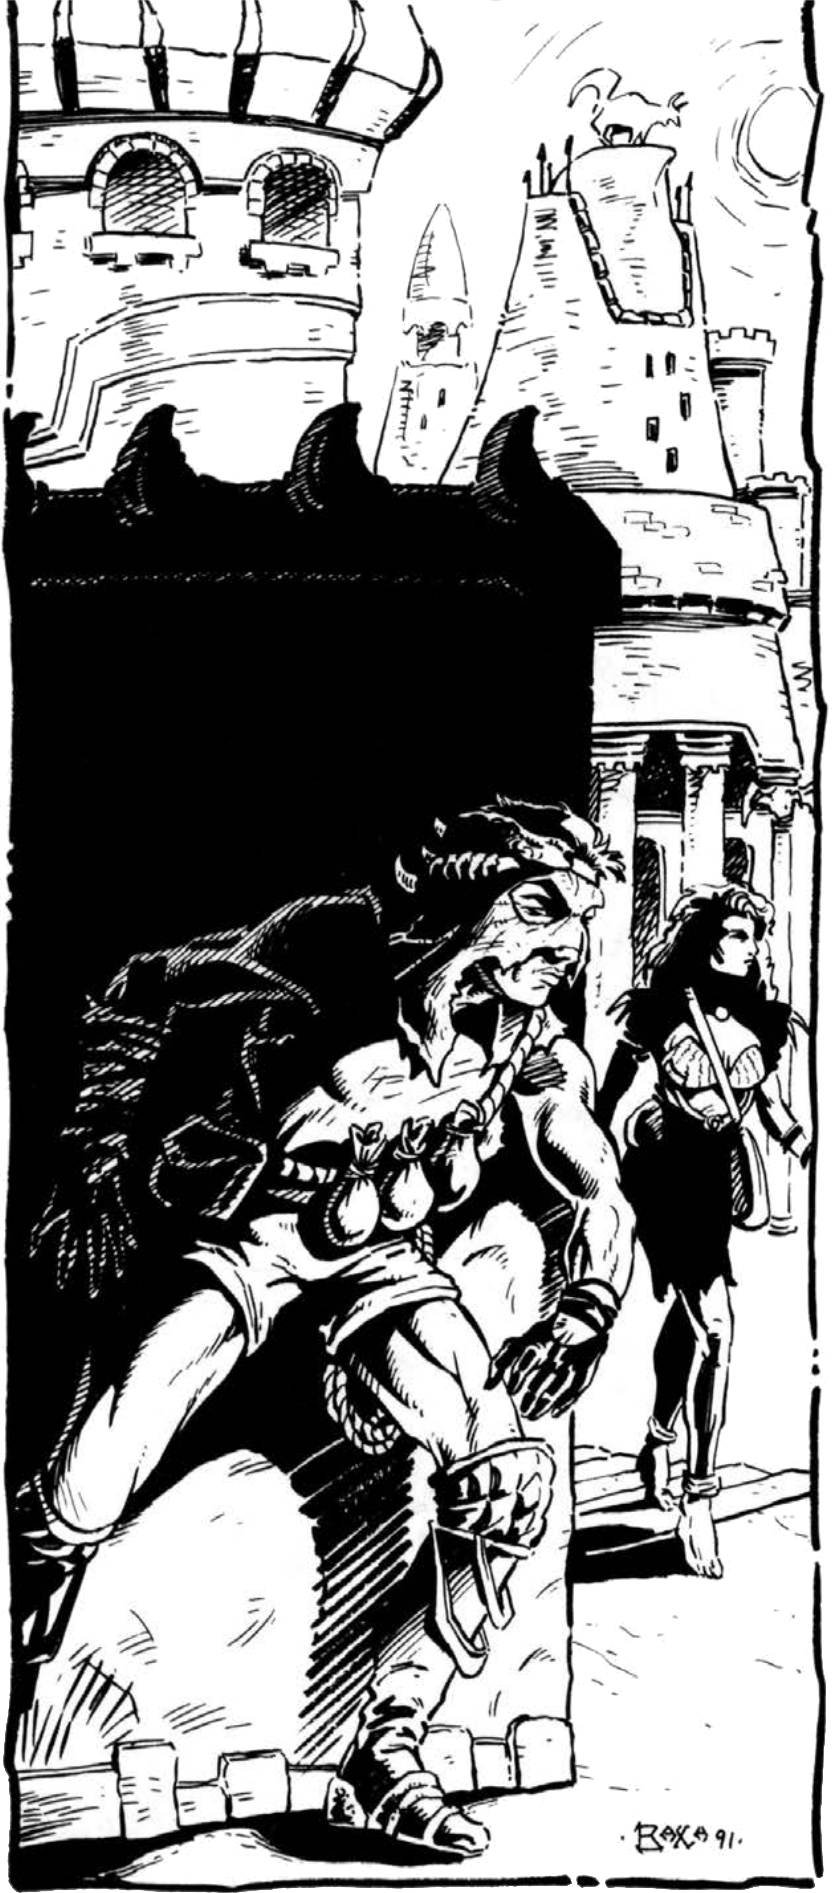
\includegraphics[width=\columnwidth]{images/rogue-1.png}
\WOTC
\end{figure}

\subsection{Making a Rogue}

A rogue can't stand up face to face with a mul warrior as well as a fighter or gladiator can. With his cunning and your various skills, however, he excels at taking the slightest opportunity and turning to his advantage. His ability to slip under the notice of an observer makes him a capable lone hunter, but his greatest strength are found through interaction with allies and foes, inside or outside, a battle---he can use his enemy`s slightest distraction to deliver a lethal blow, or ensure his party`s safe passage through a templar patrol.

\textbf{Races:} Elves, half-elves, and humans take to the rogue's skills and lifestyle with the greatest ease. Halflings, dwarves, and muls, while not commonly rogues, adapt to the class remarkably well when they take to it. Thri-kreen, pterrans, and aarakocra are usually quite adverse to the rogue class, and tend to do poorly. Half-giant rogues are unheard of except as fictional figures in comical tales around the fireside.

\textbf{Alignment:} Athasian rogues follow opportunity rather than ideals, but as many of them are lawful as chaotic. Lawful rogues tend to seek security and advancement in the service of nobles or in the ranks of the templars.

\subsection{Game Rule Information}
\textbf{Hit Die:} d6.

\subsubsection{Class Skills}
\skill{Appraise} (Int), \skill{Balance} (Dex), \skill{Bluff} (Cha), \skill{Climb} (Str), \skill{Craft} (Int), \skill{Decipher Script} (Int), \skill{Diplomacy} (Cha), \skill{Disable Device} (Int), \skill{Disguise} (Cha), \skill{Escape Artist} (Dex), \skill{Forgery} (Int), \skill{Gather Information} (Cha), \skill{Hide} (Dex), \skill{Intimidate} (Cha), \skill{Jump} (Str), \skill{Knowledge} (local) (Int), \skill{Listen} (Wis), \skill{Move Silently} (Dex), \skill{Open Lock} (Dex), \skill{Perform} (Cha), \skill{Profession} (Wis), \skill{Search} (Int), \skill{Sense Motive} (Wis), \skill{Sleight of Hand} (Dex), \skill{Spot} (Wis), \skill{Tumble} (Dex), \skill{Use Magic Device} (Cha), \skill{Use Psionic Device} (Cha), and \skill{Use Rope} (Dex).

\textbf{Skill Points per Level:} 8 + Int modifier ($\times4$ at 1st level).

\subsubsection{Class Features}
\textbf{Weapon and Armor Proficiency:} Rogues are proficient with all simple weapons, plus the bard's friend, blowgun, garrote, hand crossbow, rapier, sap, shortbow, short sword, small macahuitl, tonfa, widow's knife, and wrist razor. Rogues are proficient with light armor, but not with shields.

\textbf{Sneak Attack:} If a rogue can catch an opponent when he is unable to defend himself effectively from her attack, she can strike a vital spot for extra damage.

The rogue's attack deals extra damage any time her target would be denied a Dexterity bonus to AC (whether the target actually has a Dexterity bonus or not), or when the rogue flanks her target. This extra damage is 1d6 at 1st level, and it increases by 1d6 every two rogue levels thereafter. Should the rogue score a critical hit with a sneak attack, this extra damage is not multiplied.

Ranged attacks can count as sneak attacks only if the target is within 9 meters.

With a sap (blackjack) or an unarmed strike, a rogue can make a sneak attack that deals nonlethal damage instead of lethal damage. She cannot use a weapon that deals lethal damage to deal nonlethal damage in a sneak attack, not even with the usual $-4$ penalty.

A rogue can sneak attack only living creatures with discernible anatomies---undead, constructs, oozes, plants, and incorporeal creatures lack vital areas to attack. Any creature that is immune to critical hits is not vulnerable to sneak attacks. The rogue must be able to see the target well enough to pick out a vital spot and must be able to reach such a spot. A rogue cannot sneak attack while striking a creature with concealment or striking the limbs of a creature whose vitals are beyond reach.

\textbf{Trapfinding:} Rogues (and only rogues) can use the \skill{Search} skill to locate traps when the task has a Difficulty Class higher than 20.

Finding a nonmagical trap has a DC of at least 20, or higher if it is well hidden. Finding a magic trap has a DC of 25 + the level of the spell used to create it.

Rogues (and only rogues) can use the \skill{Disable Device} skill to disarm magic traps. A magic trap generally has a DC of 25 + the level of the spell used to create it.

A rogue who beats a trap's DC by 10 or more with a \skill{Disable Device} check can study a trap, figure out how it works, and bypass it (with her party) without disarming it.

\textbf{Evasion (Ex):} At 2nd level and higher, a rogue can avoid even magical and unusual attacks with great agility. If she makes a successful Reflex saving throw against an attack that normally deals half damage on a successful save, she instead takes no damage. Evasion can be used only if the rogue is wearing light armor or no armor. A helpless rogue does not gain the benefit of evasion.

\textbf{Trap Sense (Ex):} At 3rd level, a rogue gains an intuitive sense that alerts her to danger from traps, giving her a +1 bonus on Reflex saves made to avoid traps and a +1 dodge bonus to AC against attacks made by traps. These bonuses rise to +2 when the rogue reaches 6th level, to +3 when she reaches 9th level, to +4 when she reaches 12th level, to +5 at 15th, and to +6 at 18th level.

Trap sense bonuses gained from multiple classes stack.

\textbf{Uncanny Dodge (Ex):} Starting at 4th level, a rogue can react to danger before her senses would normally allow her to do so. She retains her Dexterity bonus to AC (if any) even if she is caught flat-footed or struck by an invisible attacker. However, she still loses her Dexterity bonus to AC if immobilized.

If a rogue already has uncanny dodge from a different class she automatically gains improved uncanny dodge instead.

\textbf{Improved Uncanny Dodge (Ex):} A rogue of 8th level or higher can no longer be flanked.

This defense denies another rogue the ability to sneak attack the character by flanking her, unless the attacker has at least four more rogue levels than the target does.

If a character already has uncanny dodge from a second class, the character automatically gains improved uncanny dodge instead, and the levels from the classes that grant uncanny dodge stack to determine the minimum rogue level required to flank the character.

\textbf{Special Abilities:} On attaining 10th level, and at every three levels thereafter (13th, 16th, and 19th), a rogue gains a special ability of her choice from among the following options.

\textit{Crippling Strike (Ex):} A rogue with this ability can sneak attack opponents with such precision that her blows weaken and hamper them. An opponent damaged by one of her sneak attacks also takes 2 points of Strength damage. Ability points lost to damage return on their own at the rate of 1 point per day for each damaged ability.

\textit{Defensive Roll (Ex):} The rogue can roll with a potentially lethal blow to take less damage from it than she otherwise would. Once per day, when she would be reduced to 0 or fewer hit points by damage in combat (from a weapon or other blow, not a spell or special ability), the rogue can attempt to roll with the damage. To use this ability, the rogue must attempt a Reflex saving throw (DC = damage dealt). If the save succeeds, she takes only half damage from the blow; if it fails, she takes full damage. She must be aware of the attack and able to react to it in order to execute her defensive roll---if she is denied her Dexterity bonus to AC, she can't use this ability. Since this effect would not normally allow a character to make a Reflex save for half damage, the rogue's evasion ability does not apply to the defensive roll.

\textit{Dune Trader:} You gain +4 competence bonus to \skill{Diplomacy} checks with regard to buying or selling goods. Furthermore, \skill{Speak Language} becomes a class skill.

\textit{False Vulnerability (Ex):} While lying prone, you are not as helpless as you appear. Opponents do not get +4 to hit you while you are prone, and you can ``kip up,'' or leap from a prone position as a free action. You do not provoke an attack of opportunity when standing up. If this ability is used with a feint action, you get a +4 circumstance bonus to your opposed Bluff roll.

\textit{Improved Evasion (Ex):} This ability works like evasion, except that while the rogue still takes no damage on a successful Reflex saving throw against attacks henceforth she takes only half damage on a failed save. A helpless rogue does not gain the benefit of improved evasion.

\textit{Looter's Luck (Ex):} You can use your \skill{Appraise} skill to instinctively identify the most valuable item in a pile of loot as a move action. The DC for this accomplishment is DC 10 + the number of items in the selection. If you cannot see the items that you are choosing from (e.g. you are trying to pickpocket someone), then a full-round action is required, and the DC rises to 15 + the number of items.

\textit{Notoriety:} The fame of your exploits precedes you in the Seven Cities; you gain +4 to all \skill{Intimidate} and \skill{Bluff} checks. Adventurers seek your fellowship; you receive a +4 to your Leadership score if you have the \feat{Leadership} feat.

\textit{Opportunist (Ex):} Once per round, the rogue can make an attack of opportunity against an opponent who has just been struck for damage in melee by another character. This attack counts as the rogue's attack of opportunity for that round. Even a rogue with the \feat{Combat Reflexes} feat can't use the opportunist ability more than once per round.

\textit{Silver Tongue (Ex):} Your constant dealing with others gives you a keen sense of how to make them believe your lies. You may attempt a retry of the Bluff skill, but with a $-5$ penalty. This ability also gives you a +2 bonus to your \skill{Disguise} skill.

\textit{Skill Mastery:} The rogue becomes so certain in the use of certain skills that she can use them reliably even under adverse conditions.

Upon gaining this ability, she selects a number of skills equal to 3 + her Intelligence modifier. When making a skill check with one of these skills, she may take 10 even if stress and distractions would normally prevent her from doing so. A rogue may gain this special ability multiple times, selecting additional skills for it to apply to each time.

\textit{Slippery Mind (Ex):} This ability represents the rogue's ability to wriggle free from magical effects that would otherwise control or compel her. If a rogue with slippery mind is affected by an enchantment spell or effect and fails her saving throw, she can attempt it again 1 round later at the same DC. She gets only this one extra chance to succeed on her saving throw.

\textit{Feat:} A rogue may gain a bonus feat in place of a special ability.

\subsection{Playing a Rogue}

Rogues run the gamut of society. Athasian rogues range from gutter snipes who prey upon the merchants and free citizens of the cities to vagabonds who steal what they can from passing caravans or merchant trains. At their best, rogues can be in the employ of the nobility, plying their trade by contract in the name of a royal household, or they can be men or women of principle and honor who steal only from the corrupt and wealthy.

There is no thieves' guild on Athasian cities. However, most Athasians rogues attempt to attract a patron. A patron is a noble or senior templar who will sponsor the rogue and protect him under his house and name. The rogue is then expected to perform certain tasks for his new master in return---including theft, spying, and even assassination.

You might adventure because you desire excitement. Someone with your smarts get bored with ordinary pursuits. Alternatively, you might have set off a life of adventure after your big heist or some political manipulation gone wrong. For some reason, you have to keep moving, and a life of adventure offers you a regular change of scenery.

All seek to exercise their abilities to grow to even greater levels of power. You are clever enough to know that there's always more to learn. Although you tend to be (dangerously) self-reliant, you understand the value of having ``friends'' and allies in your pursuits, so try to not entangle them in your web of lies and trickery until you no longer need them.

\subsubsection{Religion}

Although they are as superstitious as the next Athasian, rogues are not known for their devotion or piety. Chaotic rogues tend to get along best with religions associated with elemental air.

\subsubsection{Other Classes}

Rogues enjoy working with members of other classes so long as their own skills and are valued and treated with respect. On Athas, rogue is as honorable a profession as any other, and more honorable than some (such as wizard), and they mark for enmity anyone who describes them as a common thief.

\subsubsection{Combat}

You are at your best when you catch foes unaware. Use your skills to hide ourself so that you can employ surprise tactics. In melee, move into flanking position or use the \skill{Bluff} skill to feint in combat and drop a powerful sneak attack.

\subsubsection{Advancement}

You should assign your various skills points according to your role in your adventuring group. If the group already has someone who is good at finding traps and sneaking about, boost your ranks in social skills such as \skill{Diplomacy} and \skill{Gather Information}. High bonuses in \skill{Bluff} and \skill{Move Silently} are a must if you're going to use your sneak attacks often.

You have many good options for feats, but be sure to take \feat{Combat Expertise} and \skill{Improved Feint} to get the most out of your sneak attacks. If you are interested in having a lot of feats, it might be worthwhile to take a level of psychic warrior, since the first level of psychic warrior gives you proficiency with all types of armor, a bonus feat you could use for \feat{Combat Expertise} or \skill{Improved Feint}, and a psionic power you could use to boost your rogue skills. If you are the social type, consider becoming a \class{Dune Trader}.

\subsection{Starting Packages}
\subsubsection{The Archer}
Half-Elf Rogue

\textbf{Ability Scores:} Str 8, Dex 17, Con 12, Int 13, Wis 14, Cha 8.

\textbf{Skills:} \skill{Climb}, \skill{Disable Device}, \skill{Hide}, \skill{Listen}, \skill{Move Silently}, \skill{Open Lock}, \skill{Search}, \skill{Spot}, \skill{Tumble}.

\textbf{Languages:} Common.

\textbf{Feat:} \feat{Point Blank Shot}.

\textbf{Weapons:} Wrist razor (1d6/18--20)

Shortbow with 20 arrows (1d6/$\times$3, 18 m).

\textbf{Armor:} Studded leather (+3 AC).

\textbf{Other Gear:} Standard adventurer's kit, thieves' tools, 29 cp.

\subsubsection{The Knife in the Dark}
Elf Rogue

\textbf{Ability Scores:} Str 13, Dex 17, Con 10, Int 10, Wis 14, Cha 8.

\textbf{Skills:} \skill{Balance}, \skill{Bluff}, \skill{Disable Device}, \skill{Hide}, \skill{Listen}, \skill{Move Silently}, \skill{Open Lock}, \skill{Search}, \skill{Spot}, \skill{Tumble}.

\textbf{Languages:} Elven, Common.

\textbf{Feat:} \feat{Stealthy}.

\textbf{Weapons:} Macahuitl (1d8/19--20)

Tonfa (1d4)

Shortbow with 20 arrows (1d6/$\times$3, 18 m).

\textbf{Armor:} Studded leather (+3 AC).

\textbf{Other Gear:} Standard adventurer's kit, thieves' tools, 5 cp.

\subsubsection{The Trader}
Human Rogue

\textbf{Ability Scores:} Str 8, Dex 15, Con 10, Int 13, Wis 12, Cha 14.

\textbf{Skills:} \skill{Appraise}, \skill{Bluff}, \skill{Diplomacy}, \skill{Forgery}, \skill{Gather Information}, \skill{Knowledge} (local), \skill{Profession}, \skill{Sense Motive}, \skill{Speak Language} (cc).

\textbf{Languages:} Common.

\textbf{Feat:} \feat{Combat Reflexes}, \feat{Trader}.

\textbf{Weapons:} Longspear (1d8/$\times$3)

Wrist razor (1d6/18--20)

Light crossbow with 20 bolts (1d8/19--20, 24 m).

\textbf{Armor:} Studded leather (+3 AC).

\textbf{Other Gear:} Standard adventurer's kit, thieves' tools, 14 cp.

\subsection{Rogues on Athas}
\Quote{Going on personal experience, my one piece of advice to you is this--never trust anything with pointy ears. It'll either cheat you or try to eat you.}{Marek, human trader}

The rogue class gives a player a chance to play the archetypical trickster or scoundrel. Rogues also make great villains. By manipulating NPCs and situations the PCs encounter, or by being employed by a rival noble, an evil rogue can operate behind the scenes and trick the adventurers to his own ends.

\subsubsection{Daily Life}
The way a rogue behaves depends largely on his sense of morality. Some think nothing of adopting false identities or working as assassins for their noble patrons in exchange for silver, relying on their skills and charms to get through anything. A few other rogues find themselves driven to use their powers to help people.

\subsubsection{Notables}
The human Ramphion is the current leader of the Balican Veiled Alliance and has held the position for thirteen years, managing to rise to his title through sheer force of personality and charisma albeit not being able to cast even the simplest of cantrips. All trade lords are accomplished rogues. Master Sintha Valex is one of those, owner of large warehouses in Tyr. Frequently small quantities of the raw material are ``seeming lost'' in the warehouse, and end up being sold by Sintha to outgoing caravans to be sold in other cities of the Tablelands.

\subsubsection{Organizations}
Rogues don't organize together, but they often linger around the same places, such as the Bard's Quarter, the Elven Quarter, or Merchant House's Emporiums. A rogue joining an organization probably has a specific goal (or target) in mind and rakes a position that best allows him to attain it. A long-term commitment to such a group rarely appeals to a rogue.

\subsubsection{NPC Reactions}
Rogues make a good job about hiding their true motives and identities. Individuals who know about a rogue's true colors begin with an attitude one step more hostile than normal. Lawful clerics and templars in particular look poorly upon rogues, as does anyone who puts importance in forthrightness.

\subsubsection{Rogue Lore}
Characters with ranks in \skill{Knowledge} (local) can research rogues to learn more about them. When a character makes a skill check, read or paraphrase the following, including the information from lower DCs.

\textbf{DC 10:} Rogues are opportunists and tricksters. They employ deception and quick reflexes to get what they want.

\textbf{DC 15:} Rogues don't fight fair, if they fight at all, and their tongues are just as dangerous as their poisonous daggers.

\textbf{DC 20:} Rogues are adept at striking at vital spots when their targets are distracted, and their reflexes are quick enough to dodge most magical attacks.